\documentclass[conference]{IEEEtran}
%\IEEEoverridecommandlockouts
% The preceding line is only needed to identify funding in the first footnote. If that is unneeded, please comment it out.
\usepackage{cite}
\usepackage{amsmath,amssymb,amsfonts}
\usepackage{algorithmic}
\usepackage{graphicx}
\usepackage{textcomp}
\usepackage{xcolor}

\usepackage{attrib}

\def\BibTeX{{\rm B\kern-.05em{\sc i\kern-.025em b}\kern-.08em
    T\kern-.1667em\lower.7ex\hbox{E}\kern-.125emX}}

\begin{document}

\title{Securing Web Resources using RFID, Dynamic Groups, SIEM
  Alerting and Honeypots}

\author{\IEEEauthorblockN{Mark Deegan}
\IEEEauthorblockA{\textit{Dept.\ of Computing, Carlow Campus} \\
\textit{South East Technological University}\\
Rep.\ of Ireland\\
mark@deeganit.net}
\and
\IEEEauthorblockN{Martin Harrigan}
\IEEEauthorblockA{\textit{Dept.\ of Computing, Carlow Campus} \\
\textit{South East Technological University}\\
Rep.\ of Ireland\\
martin.harrigan@setu.ie}
}

\maketitle

\begin{abstract}
  It is a fine balance to provide employees with approved and convenient
access to corporate systems, while preventing all forms of undesired
access.  In the case of Web resources, we can better strike this
balance by cross-checking the source of the connecting device with an
employee's physical location as reported by a building's access
control system.  To this end, we assemble a collection of open-source
and proprietary components, including an RFID card reader, a directory
service with dynamic group membership, a SIEM system, and a honeypot.
We show that this assemblage can protect against internal and external
threats without imposing additional burden on employees.

Many corporate environments already have the requisite components, in
particular, a building access control system and a centralised
directory service such as Microsoft Active Directory for
authentication and authorisation.  We configure the components in a
loosely coupled architecture that utilises dynamic groups in the
directory service to store the current location of employees based on
their swipe access records.  This novel use of dynamic groups can be
combined with existing group-based rules.  We proxy all requests to
the Web resources through a load balancer that consults the directory
service and cross-checks the connection sources with the stored
location of the employees.  This defends against compromised
credential attacks from external and internal threat actors: we
illustrate this using two case studies.  The components are
interchangeable and the architecture can be adapted to many
environments.  Our approach follows the principles of the zero trust
security model and dynamic role-based access control.

\end{abstract}

\begin{IEEEkeywords}
  RFID,
  SIEM alerting,
  directory service,
  dynamic groups,
  honeypots,
  zero trust security model
\end{IEEEkeywords}

\section{Introduction}\label{sec:introduction}

To secure a Web resource in a corporate environment, there are two
modes of access to consider: an on-site user internally accessing the
resource and a remote user externally accessing the same resource.  In
the first case, the user is physically located in a building that may
be guarded by an access control system.  In the second case, the user
is located outside of those buildings.  However, attempts to access
the Web resource are often handled similarly in both cases: the
physical location of the user is ignored.  In this paper we describe a
system that combines location with credentials when securing Web
resources.  Specifically, it utilises RFID tags and readers, dynamic
groups in Microsoft Active Directory or a similar directory service,
SIEM alerting, and a honeypot.  The system provides an additional
layer of defence that imposes no extra burden on users.

\begin{quote}
  \em{There is no silver bullet solution with cybersecurity; a layered
    defence is the only viable defence.}

  \attrib{James Scott, ICIT, https://www.icitech.org/}
\end{quote}

We deployed the system using a combination of open-source and
proprietary off-the-shelf components.  The components are loosely
coupled and interchangeable.  The approach can be adapted to a variety
of corporate environments that utilise access control systems in their
buildings.  Furthermore, the system can be layered on top of existing
infrastructure.

The system distinguishes between internal and external threats and
records additional context during failed attempts to access a Web
resource.  Insider threats can be difficult and time-consuming to
detect~\cite{liu-et-al-18}.  Our system flags occasions where a
resource is accessed internally using credentials belonging to a user
that is currently operating remotely.  This runs counter to many
existing systems where internal traffic is assumed to be safer than
external traffic.

This paper is organised as follows.  In Sect.~\ref{sec:related-work}
we review related work, including RFID technology, multi-factor
authentication, dynamic role-based access control and the zero trust
security model.  In Sect.~\ref{sec:method} we describe our system:,
the high-level architecture and the various components and their
configuration.  We detail our results in Sect.~\ref{sec:results}.
Specifically, we consider two use cases: an internal user with an
external threat, and an external user with an internal threat.  In
both cases, we demonstrate the system's ability to flag threats.
Finally, we conclude in Sect.~\ref{sec:conclusion}.


\section{Related Work}\label{sec:related-work}

Amico~\cite{amico-21}


\section{Method}\label{sec:method}

In this section we describe the high-level architecture of the system.
The system comprises a variety of off-the-shelf components.  We
describe each component and its configuration.  The components are
loosely coupled and interchangeable.  For example, even though our
system relies on Microsoft Active Directory, any directory service
with dynamic groups and LDAP support will suffice.

\subsection{High-Level Architecture}

The system integrates an access control system for a building with a
directory service such as Microsoft Active Directory.  The access
control system is simulated using a Raspberry Pi and an RFID door
entry system.  When a user enters the building, they swipe their
access card.  This triggers a Python script on the Raspberry Pi that
changes the user's group from an external group to an internal group.
This signifies that they are physically located within the building.
When a user leaves the building, they swipe their access card.  This
triggers the same Python script to change the user's group from the
internal group back to the external group.  This signifies that the
user is physically located outside of the building.  The Web resource
is served by a Web server behind a reverse proxy and load balancer
(Progress Kemp LoadMaster).  This directs the traffic based on the
user's group.  It verifies that the source of the user's connection
matches their known location.  Finally, all of the components send
logs to a Security Information and Event Management (SIEM) service.
This aggregates logs, alerts and events into a centralised service
allowing investigators to perform historical and near real-time
analysis.

The system is novel in at least two aspects.  Firstly, the access
control system dynamically changes a user's group membership in the
directory service based on their physical location.  The rules for the
dynamic groups can be easily combined with existing rules.  Secondly,
the reverse proxy and load balancer direct traffic based on the user's
current group membership.  In this way, the physical location of the
user determines whether the Web resource is accessible or not.

\subsection{The Components}

Our system comprises a variety of off-the-shelf components:

\begin{itemize}
\item Microsoft Active Directory with LDAP support
\item Raspberry Pi connected to an RFID door entry system (see
  Fig.~\ref{fig:raspberry-pi-rfid})
\item Progress Kemp LoadMaster~\cite{progress-kemp-loadmaster-xx}
\item Progress WhatsUp Gold~\cite{progress-kemp-whatsup-gold-xx}
\item Web servers (Apache HTTP Server)
\end{itemize}

We describe each component and its configuration in the following
subsections.

\subsubsection{Microsoft Active Directory With LDAP Support}

\begin{figure}
  \centerline{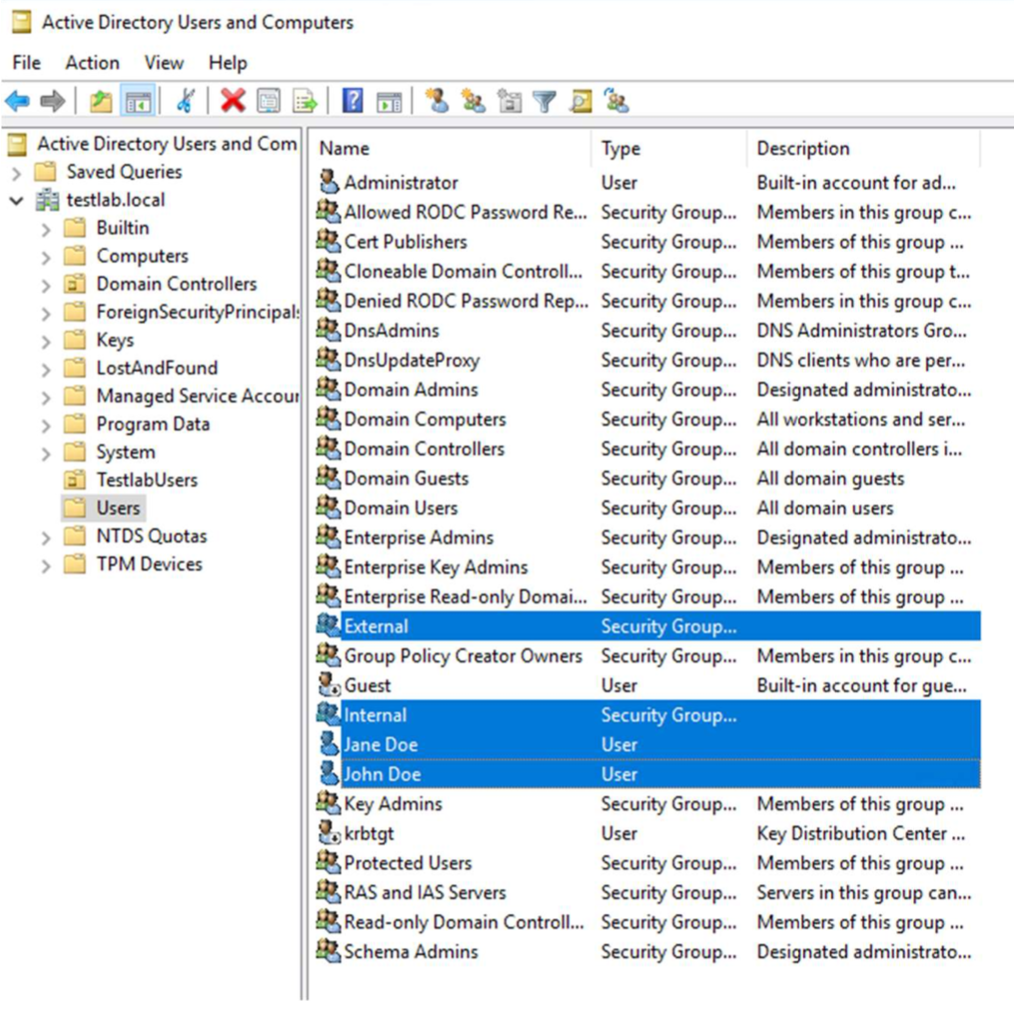
\includegraphics[width=\columnwidth]{img/active-directory}}
  \caption{We created two users, Jane Doe and John Doe, and two
    groups, Internal and External, in Microsoft Active Directory.  We
    also enabled LDAP support.}\label{fig:active-directory}
\end{figure}

We used Microsoft Windows Server 2019 to run a Domain Controller (DC)
(\texttt{d1.testlab.local}) for our domain (\texttt{testlab.local}).
This is the primary DC for the scenario and it was setup to host
Active Directory (AD) with LDAP support and the Domain Name System
(DNS).  AD provides authentication and authorisation services, and
allows administrators to manage network resources centrally.  To
ensure that the requests for the Web resources go to the appropriate
services on the Progress Kemp LoadMaster, we created corresponding DNS
delegations.  This is important as we wanted the external requests to
be pointed to the external resources and the internal requests to be
pointed to the internal resources.  It also allows the LoadMaster to
perform service health checks before responding to DNS requests thus
preventing IP addresses being returned when resources are unavailable.
We added two users, Jane Doe and John Doe, and two groups, Internal
and External, to AD (see Fig.~\ref{fig:active-directory}).

\subsubsection{Raspberry Pi and RFID Door Entry System}

\begin{figure}
  \centerline{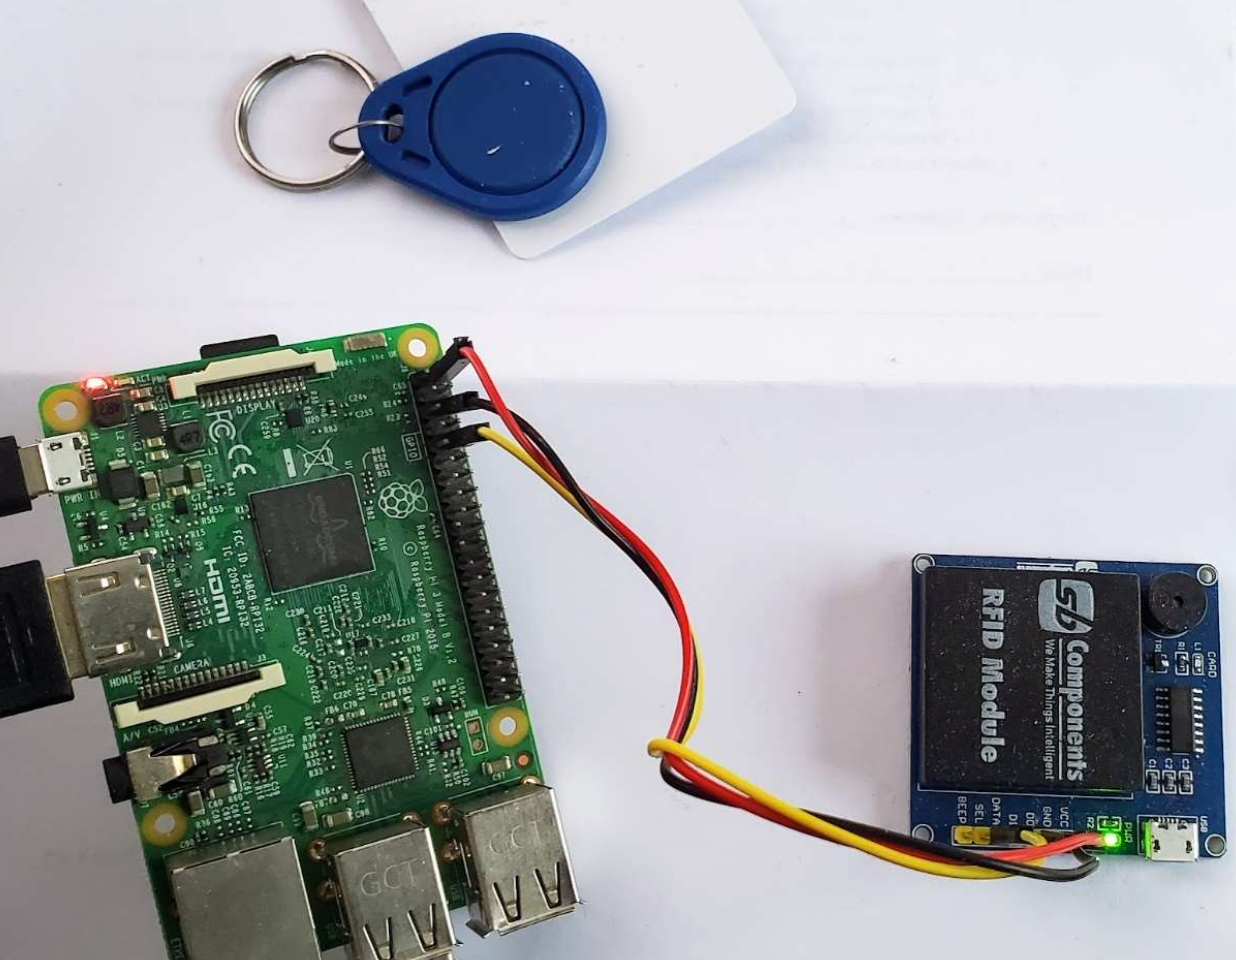
\includegraphics[width=\columnwidth]{img/raspberry-pi-rfid}}
  \caption{The Raspberry Pi was connected to an RFID door entry
    system.  We created a Python script that read the identification
    details from swiped cards and interacted with Active
    Directory.}\label{fig:raspberry-pi-rfid}
\end{figure}

The Raspberry Pi is connected to an RFID door entry system.  When a
user performs a card swipe, a Python script running on the Raspberry
Pi reads the identification details from the card and remotely changes
the group membership of the user in AD.  If the user is entering the
building their group membership is changed from External to Internal;
if they are leaving the building it is changed from Internal to
External.  The Python script uses the
\texttt{ldap3}\footnote{https://ldap3.readthedocs.io/} package to
interact with AD.  It logs all events to a SIEM service (see
Sect.~\ref{sec:wug}).

\subsubsection{Progress Kemp LoadMaster}

Progress Kemp LoadMaster (LM) is a reverse proxy and load
balancer~\cite{progress-kemp-loadmaster-xx}.  It has many capabilities
but for this scenario we are interested in the Edge Security Pack
(ESP), the source IP blacklist from the GEO component, and the Web
Application Firewall (WAF).  We use the ESP for Single Sign-On (SSO)
for HTTP(S) services and to communicate with AD during login and to
query group memberships.  This pre-authenticates a user before they
gain access to a resource.  We also enabled \textit{group steering} on
the ESP: this allows LM to send traffic to particular services based
on their group membership in AD and goes beyond the normal use of
groups to simply allow or deny access.

\begin{figure*}
  \centerline{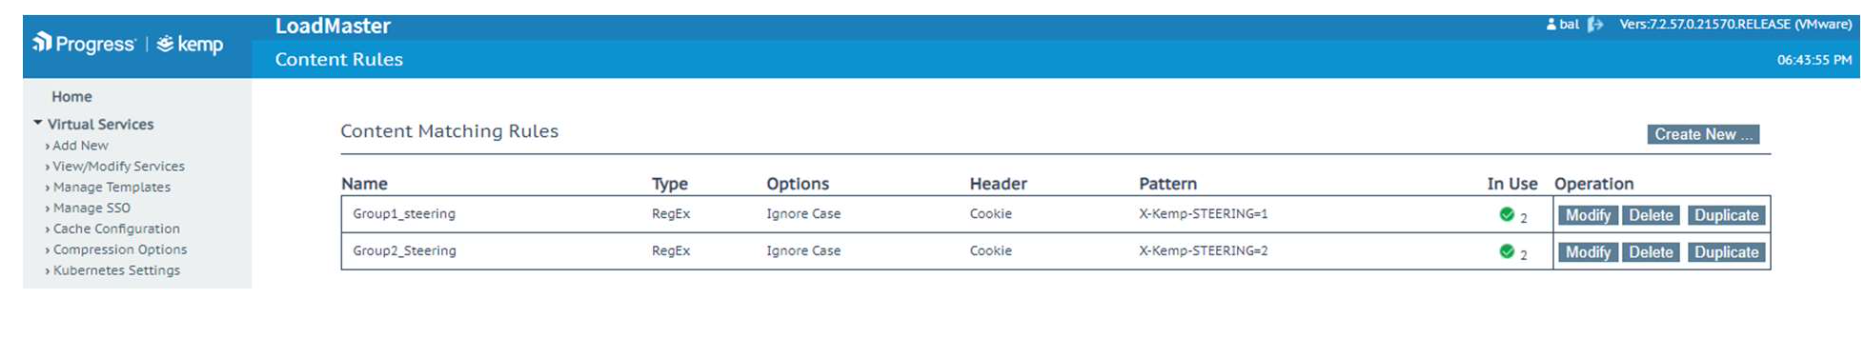
\includegraphics[width=\textwidth]{img/loadmaster-pcre-rules}}
  \caption{LoadMaster can direct traffic based on steering groups: we
    created two such groups, one for internal traffic and one for
    external traffic.}\label{fig:loadmaster-pcre-rules}
\end{figure*}

We created two steering groups associated with the Internal and
External groups in AD.  We created Perl Compatible Regular Expression
(PCRE) rules to match the authorisation headers and steer the requests
to the appropriate services (see
Fig.~\ref{fig:loadmaster-pcre-rules}).

The login page that is displayed by the ESP is the same for both
\textit{valid} and \textit{invalid} access attempts.  A valid access
attempt occurs when a user's group and request are both internal or
both external; otherwise the access attempt is invalid.  In both cases
a log is sent to a SIEM service (see Sect.~\ref{sec:wug}).  This helps
with threat hunting as a threat actor will see the same login page for
the honeypot as for the valid site.  The honeypot can gather the
details of the access attempt without being discovered.

\begin{figure*}
  \centerline{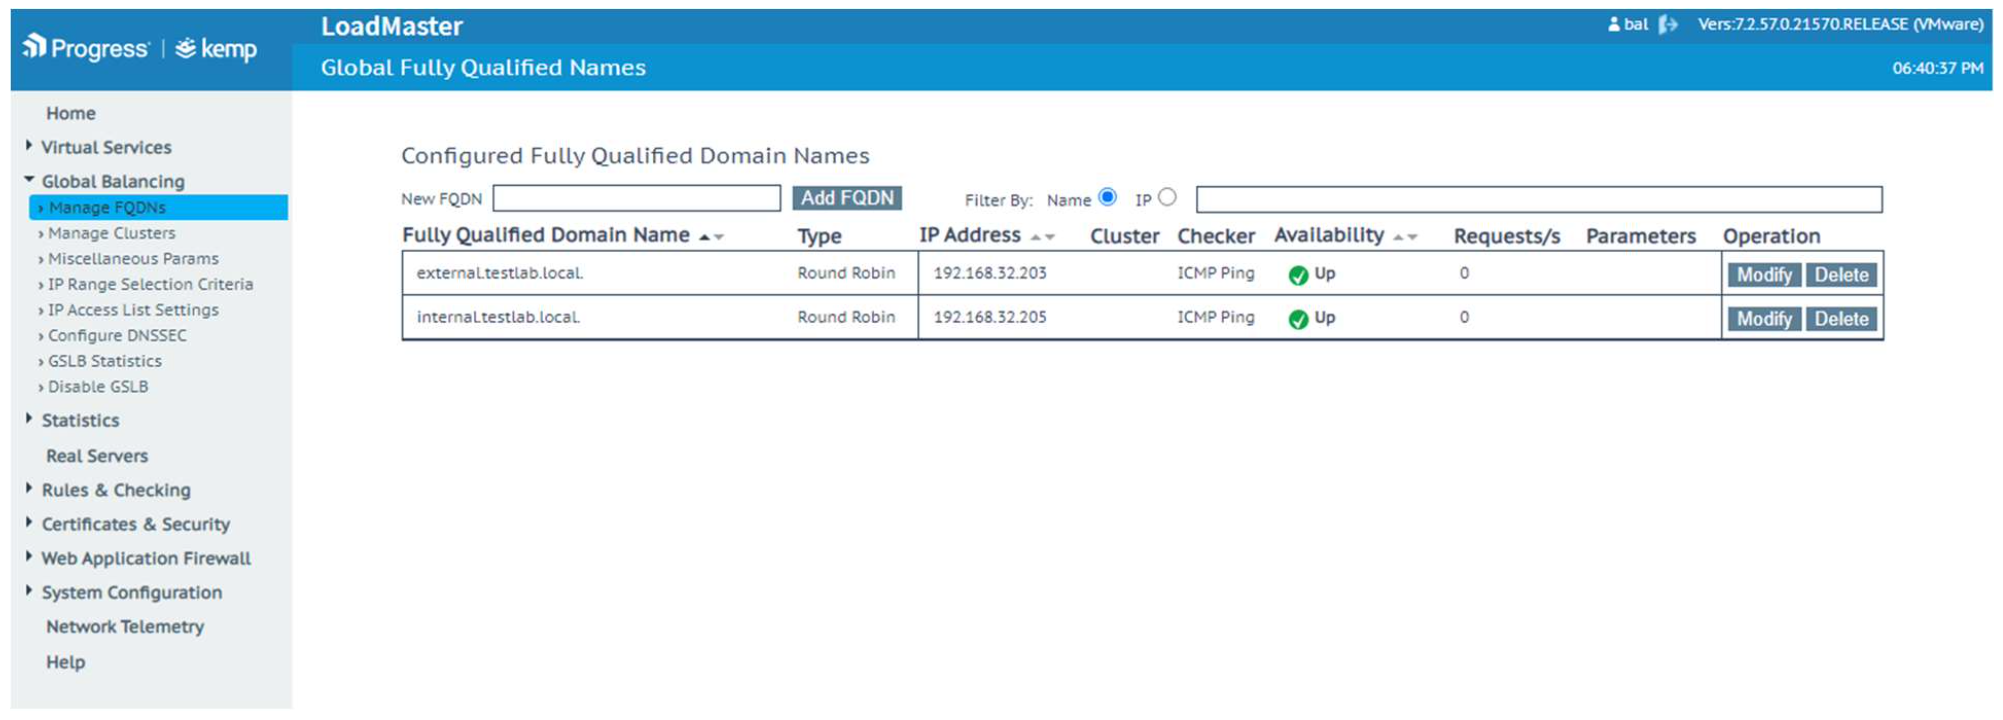
\includegraphics[width=\textwidth]{img/loadmaster-geo}}
  \caption{We configured two FQDNs for \texttt{internal.testlab.local}
    and \texttt{external.testlab.local} using LoadMaster's GEO
    component.}\label{fig:loadmaster-geo}
\end{figure*}

The GEO component performs DNS resolution and service health checks
before returning a result.  We created GEO DNS entries for
\texttt{internal.testlab.local} and \texttt{external.testlab.local}
(see Fig.~\ref{fig:loadmaster-geo}).  We also used an IP blacklist
that is updated daily to withhold DNS results from anyone on the list.

\begin{figure*}
  \centerline{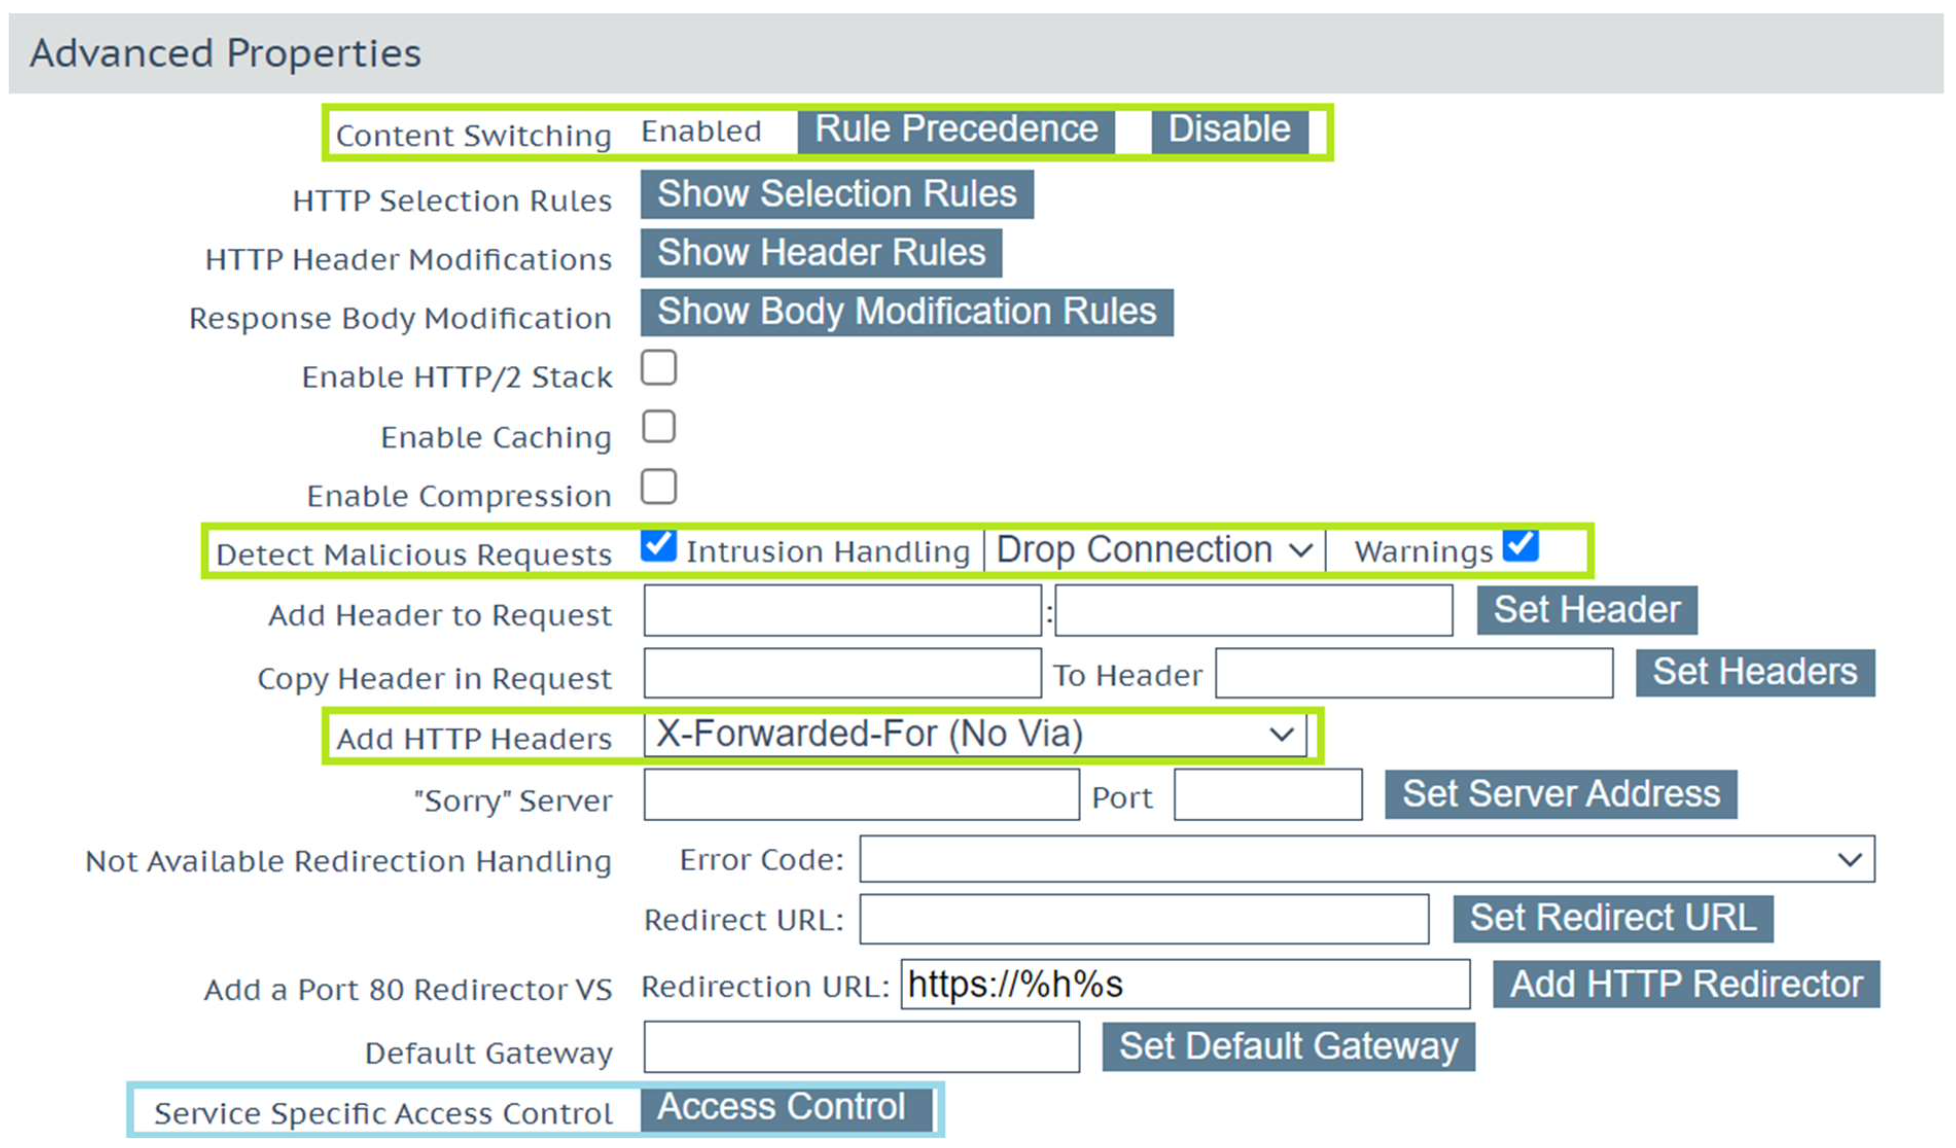
\includegraphics[width=\textwidth]{img/loadmaster-ids-ips}}
  \caption{We enabled Content Switching in LoadMaster so that the PCRE
    engine is enabled for group steering (first green rectangle).  We
    enabled IDS/IPS as an additional layer of defence (second green
    rectangle).  We also added \texttt{X-Forwarded-For} HTTP headers
    to enable the Flask application (honeypot) to easily record the
    originating IP addresses of invalid access attempts (third green
    rectangle).  We could also enable the Service Specific Access
    Control to prevent access via whitelists and blacklists (blue
    rectangle).  This was not enabled during our
    tests.}\label{fig:loadmaster-ids-ips}
\end{figure*}

Additionally, we enabled the Intrusion Detection System (IDS) and
Intrusion Prevention Systems (IPS) on LM.  This includes rules defined
by the SNORT community~\cite{cisco-snort-xx} and enables the SNORT
rule filtering on the Layer 7 HTTP engine to check for any known bad
requests.  Figure~\ref{fig:loadmaster-ids-ips} shows the configuration
highlighted in green.  There is also an option to prevent access via
whitelists and blacklists highlighted in blue.

Finally, we enabled the Web Application Firewall (WAF) and the Open
Web Application Security Project (OWASP) core rule set.  This rule set
performs anomaly scoring and identifies, for each request, the
probability that it is malicious.  The core rule set protects against
SQL injection, cross-site scripting, remote code execution, buffer
overflows, known vulnerabilities, and many other attack vectors.  We
configured the WAF with source IP reputation blocking enabled which
uses a global IP reputation list that is updated daily.  Using the
MaxMind~\cite{maxmind-xx} and the GEO component, it identifies the
country of the source request and it can be configured to block
specific countries or regions.

\subsubsection{Web Servers}

Our Web servers are hosted on virtual machines running Debian and a
default installation of the Apache HTTP Server.  The landing page is
our ``valid access'' page and represents our secured Web resource.
The ``invalid access'' page is served by a Flask
application\footnote{https://flask.palletsprojects.com/}.  It records
the usernames and source IP addresses of all requests and sends those
details to a SIEM service (see next section).  The details are
extracted from the authorisation and \texttt{X-Forwarded-For} headers.
The Flask application is a honeypot: it reports to a user that a
requested resource is unavailable rather than reporting that an access
attempt was invalid.

\subsubsection{Progress WhatsUp Gold}\label{sec:wug}

\begin{figure*}
  \centerline{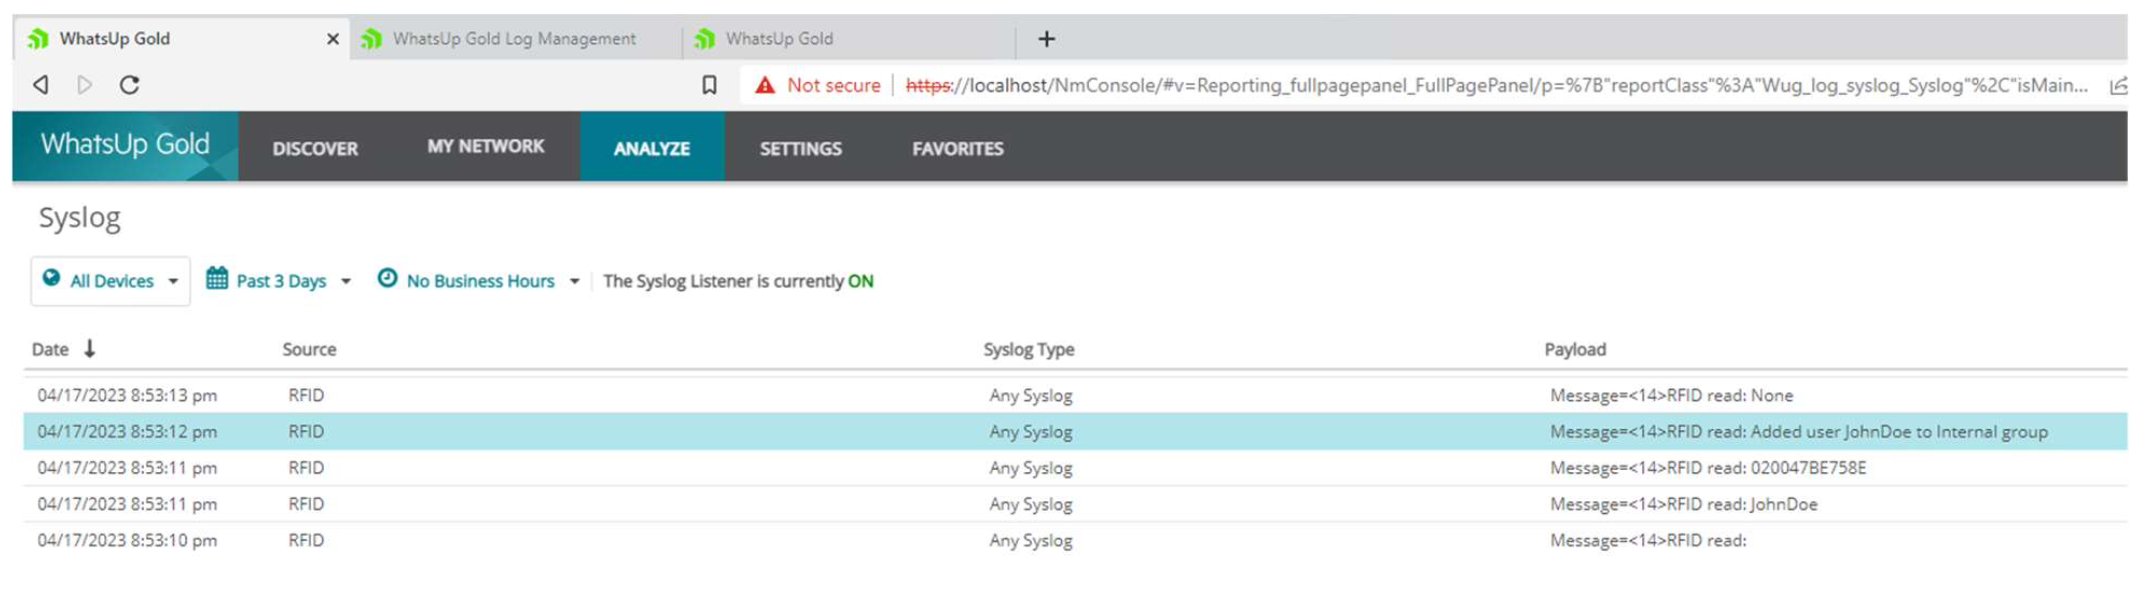
\includegraphics[width=\textwidth]{img/whatsup-gold}}
  \caption{We record all events using WhatsUp Gold.  In the above we
    observe a user changing group (from External to Internal) as they
    swipe their access card when entering a
    building.}\label{fig:whatsup-gold}
\end{figure*}

The Raspberry Pi, LM, and Flask application send logs to a SIEM
service.  We use Progress WhatsUp Gold (WUG) (see
Fig.~\ref{fig:whatsup-gold}) to gather and manage all device log data.
In normal operation the events from the Raspberry Pi, RFID door entry
system, and LM are logged.  We use the Syslog protocol, a standard
network-based logging protocol, for all events.  In cases where a
user's credentials may be compromised, the Flask application logs an
event with high priority.


\section{Results}\label{sec:results}

We configured the system as described in the previous section.  The
goal of the study was to show the feasibility of the integration
between the various components, and to demonstrate that dynamic group
membership based on real-world location can secure Web resources.  We
performed two tests (Sect.~\ref{sec:case-one} and
Sect.~\ref{sec:case-two}) to demonstrate this aspect of the system.

\subsection{Internal User with External Threat}\label{sec:case-one}

In the first case the user, John Doe, enters his office during normal
working hours and swipes his access card at the door using an RFID
tag.  His group membership is set to Internal and the user can then
access the resource internally.  Meanwhile an external threat actor
attempts to login from outside the office while the user is at work.
They are denied access and they have their IP address logged to the
SIEM service (WUG) as a breach attempt.  This requires no extra
overhead on the user to secure his credentials.  The timeline of
events is as follows:

\begin{figure*}
  \centerline{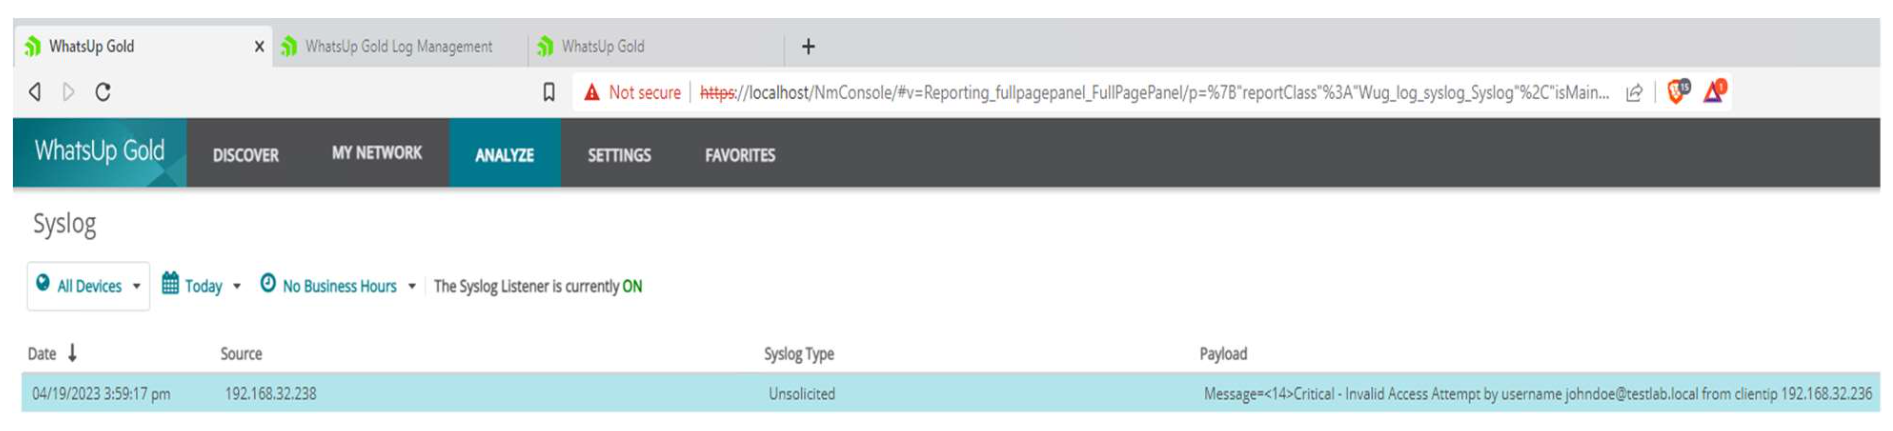
\includegraphics[width=\textwidth]{img/whatsup-gold-alert}}
  \caption{...}\label{fig:whatsup-gold-alert}
\end{figure*}

\begin{enumerate}
\item John Doe enters his office and swipes his access card.
\item The user's group membership is changed from External to
  Internal.  This event is logged to the SIEM service from the
  Raspberry Pi.
\item When the user gets to his desk they access the Web resource
  internally.
\item The DNS points to the LM for DNS resolution of the Web resource
  and since it is an internal request the user is sent to the internal
  service.
\item The ESP requires the user to login.
\item The user's group membership is checked by the ESP SSO system and
  they are connected to the appropriate Web resource.
\item An external threat actor attempts to access the Web resource
  using John Doe's credentials.
\item The DNS points the threat actor to the LM for DNS resolution.
\item Using the correct credentials, the external threat actor logs in
  via the ESP SSO page.
\item The group membership is read as Internal, but the source is
  external, so the threat actor is directed to a ``server
  unavailable'' page and their IP address is logged to the SIEM
  service (see Fig.~\ref{fig:whatsup-gold-alert}).
\end{enumerate}

\subsection{External User with Internal Threat}\label{sec:case-two}

In the second case we are concerned with internal threats: rather than
credentials being leaked externally, they are accessed by a threat
internally, e.g., someone who may have physical access to the user's
desk.  The user, Jane Doe, leaves the office for lunch and swipes her
access card on the RFID reader on the way out.  Her group membership
is set to External.  Meanwhile an internal threat actor attempts to
login from inside the office while the user is away.  They are denied
access and an event is logged to the SIEM service (WUG) as a breach
attempt.  The timeline of events is as follows:

\begin{enumerate}
\item Jane Doe leaves her office and swipes his access card.
\item The user's group membership is changed from Internal to
  External.  This event is logged to the SIEM service from the
  Raspberry Pi.
\item An internal threat actor attempts to access the Web resource
  using Jane Doe's credentials.
\item The DNS points the threat actor to the LM for DNS resolution.
\item Using the correct credentials, the internal threat actor logs in
  via the ESP SSO page.
\item The group membership is read as External, but the source is
  internal, so the threat actor is directed to a ``server
  unavailable'' page.  The event is logged to the SIEM service.
\end{enumerate}


\section{Conclusion}\label{sec:conclusion}

Our system demonstrates the feasibility of securing Web resources in a
corporate environment based on the physical location of users as
implied by a building access control system.  The system uses dynamic
group membership in a directory service such as Active Directory to
store the last known physical location of users.  It updates their
locations as they swipe their access cards on a RFID reader.  All
events are logged to a SIEM service, and, in the case of an invalid
access attempt, the threat actor is directed to a honeypot that flags
the event as high priority.  The system can prevent both internal and
external threats without placing additional burden on users.  It is
constructed from open-source and proprietary off-the-shelf components
in a vendor-neutral manner.  It adds a additional layer of defence
when securing Web resources.

Our approach follows the principles of zero trust architecture (ZTA)
as outlined in Sect.~\ref{sec:related-work}.  The physical location of
a user determines the appropriate defence around a Web resource.
Additionally, dynamic group membership is an example of role-based
access control (RBAC), and specifically, dynamic role-based access
control (DRBAC) (see Sect.~\ref{sec:related-work}): a user's role is
automatically adjusted based on context.  The real-time evaluation of
the context is performed by the directory service.  Our system is a
proof-of-concept but it can be extended in many ways.  For example, we
could incorporate temporal information from calendars and attendance
trackers, e.g., holidays, business travel, medical leave, etc.  We
could use fine-grained location information~\cite{kriplean-et-al-07}
and include geospatial data from mobile devices and laptops.



\bibliographystyle{IEEEtran}
\bibliography{bib/main}

\end{document}
